%----------------------------------------------------------------------------------------
%	CHAPTER - SUGGESTION
%----------------------------------------------------------------------------------------

\chapter{Suggestion}

\label{ChapterSuggestion}

The in Chapter \ref{DSRCycle} discussed \gls{dsr} cycle from \cite{Vaishnavi2008} and \cite{Hevner2010} defines \textit{Suggestion} as the next step after \textit{Awareness of Problem}. \cite{Vaishnavi2008} define the \textit{Suggestion} phase as a creative step in which new functionality is envisioned to form a tentative design for the development of the artefact. \cite{Vaishnavi2008} further specify the output as a constructed theory that addresses the identified problem, which can include new ideas and concepts, new methods, and new models that in the end shall be validated with the development of the artefact.

%----------------------------------------------------------------------------------------
%	SECTION 1
%----------------------------------------------------------------------------------------

\section{Introduction}

In a first step, the end goals of the design are defined, which will be relevant for the evaluation in Chapter \ref{ChapterEvaluation}. Then the individual views of presentation (e.g. an overview and detail view) are defined as well as the navigation between them. As the third step, the visualisation of the individual views are defined before finally the interaction patterns (action/reaction) can be mapped to them. With this information, it will be possible to give an answer to the fourth \gls{srq}:
\begin{framed}
 	\textit{\gls{srq} 4: \srqfourtext}
\end{framed}
Building up on this, the \textit{Development} phase will then be discussed in Chapter \ref{ChapterDevelopment}.


%----------------------------------------------------------------------------------------
%	SECTION 2
%----------------------------------------------------------------------------------------

\section{Goals of the Design}

In order to define the goals of the design, the specific characteristics of \gls{vr} itself and the to be visualized data have to be considered. In this thesis, the goals are defined either as \glspl{mdg} for the more overarching goals, or as \glspl{sdg} which are focussing rather on specific areas. In the following sub-chapters, these characteristics are discussed in more detail and the individual goals are defined over the three main categories: \gls{vr}, data, and visualisation.
\newcounter{MainDesignGoalCounter} % Create two new counters
\newcounter{SubDesignGoalCounter}
\stepcounter{MainDesignGoalCounter} % Increase both values from 0 to 1
\stepcounter{SubDesignGoalCounter}

%-----------------------------------
%	SUBSECTION 1
%-----------------------------------
\subsection{VR-specific Goals}

The goals that are derived from \gls{vr} itself, are more high-level since they can be applied to any \gls{vr} application independent of what its purpose is. Therefore, the three important characteristics of \gls{vr} as defined by \cite{Stone1994} and discussed in Chapter \ref{SubSectionVisualisationManipulation} are considered as an integral part of the design. These characteristics can be summarized in the following three keywords: Action/Reaction, Immersion and Spatial. Based on these, the first \glspl{mdg} from a \gls{vr} perspective can be derived and further described with examples:
\begin{itemize}[noitemsep,nolistsep]
	\item \textbf{\gls{mdg} \arabic{MainDesignGoalCounter}:} High interactivity with tightly coupled actions/reactions \newline
		\textit{Example: No slow animations, no timed events, or any other change in scenery without a trigger from the user}
		\stepcounter{MainDesignGoalCounter}
	\item \textbf{\gls{mdg} \arabic{MainDesignGoalCounter}:} The user is part of the \gls{ve} and thus is able to 'travel' around the visualisations \newline
		\textit{Example: Movement at free will, and no outside view, or third-person \gls{pov}}
		\stepcounter{MainDesignGoalCounter}
	\item \textbf{\gls{mdg} \arabic{MainDesignGoalCounter}:} The design is intended for \gls{vr} and thus in full 3D \newline
		\textit{Example: No flattened two-dimensional representation in 3D space}
		\stepcounter{MainDesignGoalCounter}
\end{itemize}
In addition to the above characteristics, another goal has to be that the design should not rely on specific \gls{vr}-hardware, but rather define them in a more abstract way as to what the individual hardware items should be capable of. Since this topic is only important for the \gls{vr} input devices and potentially the \gls{hmd} but not the visualisation itself, it is considered as a \gls{sdg}.
\begin{itemize}[noitemsep,nolistsep]
	\item \textbf{\gls{sdg} \arabic{SubDesignGoalCounter}:} The design is independent of specific \gls{vr} hardware \newline
		\textit{Example: No direct references to specific hardware, but rather what the hardware has to be capable of (requirements)}
		\stepcounter{SubDesignGoalCounter}
\end{itemize}
From a \gls{vr} perspective, the important areas can all be covered with the above defined goals. The main aspects of the design are depending on what data is used and thus is discussed in the following sub-chapter.


%-----------------------------------
%	SUBSECTION 2
%-----------------------------------

\subsection{Data-specific Goals}

The data set that is used for this thesis is shown in Appendix \ref{AppendixA} and contains information about categorized financial expenses of one year. The focus for the data-specific goals is put on this specific data-set and might only partially be applicable to other data sets. Since the goal of this thesis is to enhance the current interaction with the data, the presentation should provide \textbf{at least} the same amount of information to the user.
\begin{itemize}[noitemsep,nolistsep]
	\item \textbf{\gls{mdg} \arabic{MainDesignGoalCounter}:} The design provides at least the same information as existing applications \newline
		\textit{Example: View on individual months or the whole year, summed-up expenses based on their category, or easy comparison of different categories (based on total amount)}
		\stepcounter{MainDesignGoalCounter}
\end{itemize}
In order to provided an added value to the user, further quality of life features such as direct access to the underlying transactions, the filtering of individual categories, or the display of a (spending) trend are considered. They support the main functionality of data exploration by rendering certain tasks easier and more convenient for the user. Due to this supporting aspect, this is considered as a \gls{sdg}.
\begin{itemize}[noitemsep,nolistsep]
	\item \textbf{\gls{sdg} \arabic{SubDesignGoalCounter}:} The design includes new quality-of-life features \newline
	\textit{Example: Direct access to underlying transactions, filtering of individual categories, or the display of a (spending) trend-line}
	\stepcounter{SubDesignGoalCounter}
\end{itemize}


%-----------------------------------
%	SUBSECTION 3
%-----------------------------------

\subsection{Visualisation Goals}

The \gls{vism} from \cite{Shneiderman2005} (see Chapter \ref{SubSectionVISM}) has proven to be a solid base design principle whenever the to be executed work is focussed on finding information. This matches the situation of analysing ones financial expenses very well and thus is seen as one of the \gls{mdg} from a visualisation perspective.
\begin{itemize}[noitemsep,nolistsep]
	\item \textbf{\gls{mdg} \arabic{MainDesignGoalCounter}:} The design follows the \gls{vism} \newline
		\textit{Overview first, zoom and filter, then details-on-demand}
		\stepcounter{MainDesignGoalCounter}
\end{itemize}
In addition, the design should also include the improvements from \gls{vism} 2.0 by adhering to the seven main tasks as defined by \cite{Stauffer2016} and shown in Figure \ref{fig:vism2}. The three support tasks (i.e. History, Extract, and Collaboration) are not considered to be relevant for the prototype since they are only support tasks and thus not relevant for the main functionality. They however could become relevant for future research in this area. Since version 2.0 is an enhancement to the existing mantra, it is deemed as a \gls{sdg}.
\begin{itemize}[noitemsep,nolistsep]
	\item \textbf{\gls{sdg} \arabic{SubDesignGoalCounter}:} The design adheres to the seven main tasks of \gls{vism} 2.0 \newline
		\textit{Main Tasks: Overview, Zoom In, Zoom Out, Filtering, Relate, Details, and Multi View}
		\stepcounter{SubDesignGoalCounter}
\end{itemize}

% For the "conclusion", we have to remove "1" from the counter again:
\addtocounter{MainDesignGoalCounter}{-1}
\addtocounter{SubDesignGoalCounter}{-1}
% -------------------------------------------


%-----------------------------------
%	SUBSECTION 4
%-----------------------------------

\subsection{Conclusion}

With this, all goals that are relevant for the design have been covered and summarized into \arabic{MainDesignGoalCounter} \glspl{mdg} and \arabic{SubDesignGoalCounter} \glspl{sdg}. They will be primarily relevant for the other chapters of the \textit{Suggestion} phase, but also for the \textit{Development} and \textit{Evaluation} phase. \newline
The next chapter focuses on the definition of the individual views that are available, and how the navigation in between them is defined.


%----------------------------------------------------------------------------------------
%	SECTION 3
%----------------------------------------------------------------------------------------

\section{View Definition and Navigation Map}

\newcounter{ViewCounter} % Create a new counter
\stepcounter{ViewCounter} % Increase value from 0 to 1

In a first step, the different individual views are defined, before a navigation map can be defined that shows what transitions can be possible from one view to another.


%-----------------------------------
%	SUBSECTION 1
%-----------------------------------

\subsection{View Definition}

As defined in \gls{mdg} 5 and \gls{sdg} 3, the \gls{vism} respectively the \gls{vism} 2.0 is part of the core design principle for the prototype of this thesis. \cite{Shneiderman1996} defined the following mantra as the fundamental visual design guideline:
\begin{framed}
	\textit{Overview first, zoom and filter, then details-on-demand}
\end{framed}
This mantra already clearly distinguishes between to main views: overview and detail. By looking at the \textit{Overview} perspective in regards to the financial expenses, this either could be a summary of the current year, or a bit more detailed the summary of the current month, or even just a 'blank page' where the first entry point has to be chosen from. The last interpretation goes in the direction of what \cite{Neil2006} claimed to be one of the big downfalls of \gls{vism}, that a user might already know what data he wants to see and thus does not want to start on an overview and then dig down to the details. Due to the increased available space in \gls{vr}, it however becomes possible to fulfil all of these demands by presenting all three options next to each other. This also relates to the idea of the \textit{Multi View} which is one of the seven main tasks of \gls{vism} 2.0 as defined by \cite{Stauffer2016}. This allows to define the first three views:
\begin{itemize}[noitemsep,nolistsep]
	\item \textbf{View \arabic{ViewCounter}:} Overview of (current) year
	\stepcounter{ViewCounter}
	\item \textbf{View \arabic{ViewCounter}:} Overview of (current) month
	\stepcounter{ViewCounter}
	\item \textbf{View \arabic{ViewCounter}:} Selection of different year
	\stepcounter{ViewCounter}
\end{itemize}
The next main task from \gls{vism} 2.0 which is also part of the original mantra is about \textit{Filtering}, which in this (data) context can be applied to the different main categories as shown in Table \ref{tbl:financialcategories} in Chapter \ref{ChapterIntroduction}. To further adhere to the \textit{Multi View} task, the filtering is put in an additional view to not interfere with the actual data visualisation.
\begin{itemize}[noitemsep,nolistsep]
	\item \textbf{View \arabic{ViewCounter}:} Filtering of main categories
	\stepcounter{ViewCounter}
\end{itemize}

Continuing the main tasks from \gls{vism} 2.0, we come to \textit{Details} which for the data set that is used in this thesis is a single individual financial transaction. This additional view provides all detailed information about the transaction, from date over amount and recipient to the categories. Since it however is not directly possible to go from a grouped view into a single transaction, an intermediate view that lists all transactions has to be added.
\begin{itemize}[noitemsep,nolistsep]
	\item \textbf{View \arabic{ViewCounter}:} Overview of filtered financial transactions
	\stepcounter{ViewCounter}
	\item \textbf{View \arabic{ViewCounter}:} Details of a single financial transaction
	\stepcounter{ViewCounter}
\end{itemize}


% For the "conclusion", we have to remove "1" from the counter again:
\addtocounter{ViewCounter}{-1}
% -------------------------------------------

This concludes all the relevant views for the design. This is also in correspondence with \gls{mdg} 4 that states that \textbf{at least} the same functionality has to be provided as it is done in current 2D applications. \newline
In the next step, the navigation between them are defined which covers the \textit{Relate}, \textit{Zoom In} and \textit{Zoom Out} tasks from the \gls{vism} 2.0.


%-----------------------------------
%	SUBSECTION 2
%-----------------------------------

\subsection{Navigation Map}

After the definition of all views, the navigation in between them has to be defined. The base principle for the definition is again the \gls{vism} to make sure it is possible to navigate from the overview into the detail view. Figure \ref{fig:navigationmap} shows the proposed navigation map with all previously defined views. The four green views (1, 2, 5, and 6) are considered the main views where actual data is presented, whereas the two blue views (3 and 4) are considered the supporting views that do not display any actual data, but rather help with the navigation between the main screens. The green arrows indicate the main navigation flow, whereas the blue ones are more influential flows in terms of  altering the green views. With these additional flows, the \gls{sdg} 2 is also covered to provide additional quality of life features. \newline
\begin{figure}[h]
	\begin{center}
		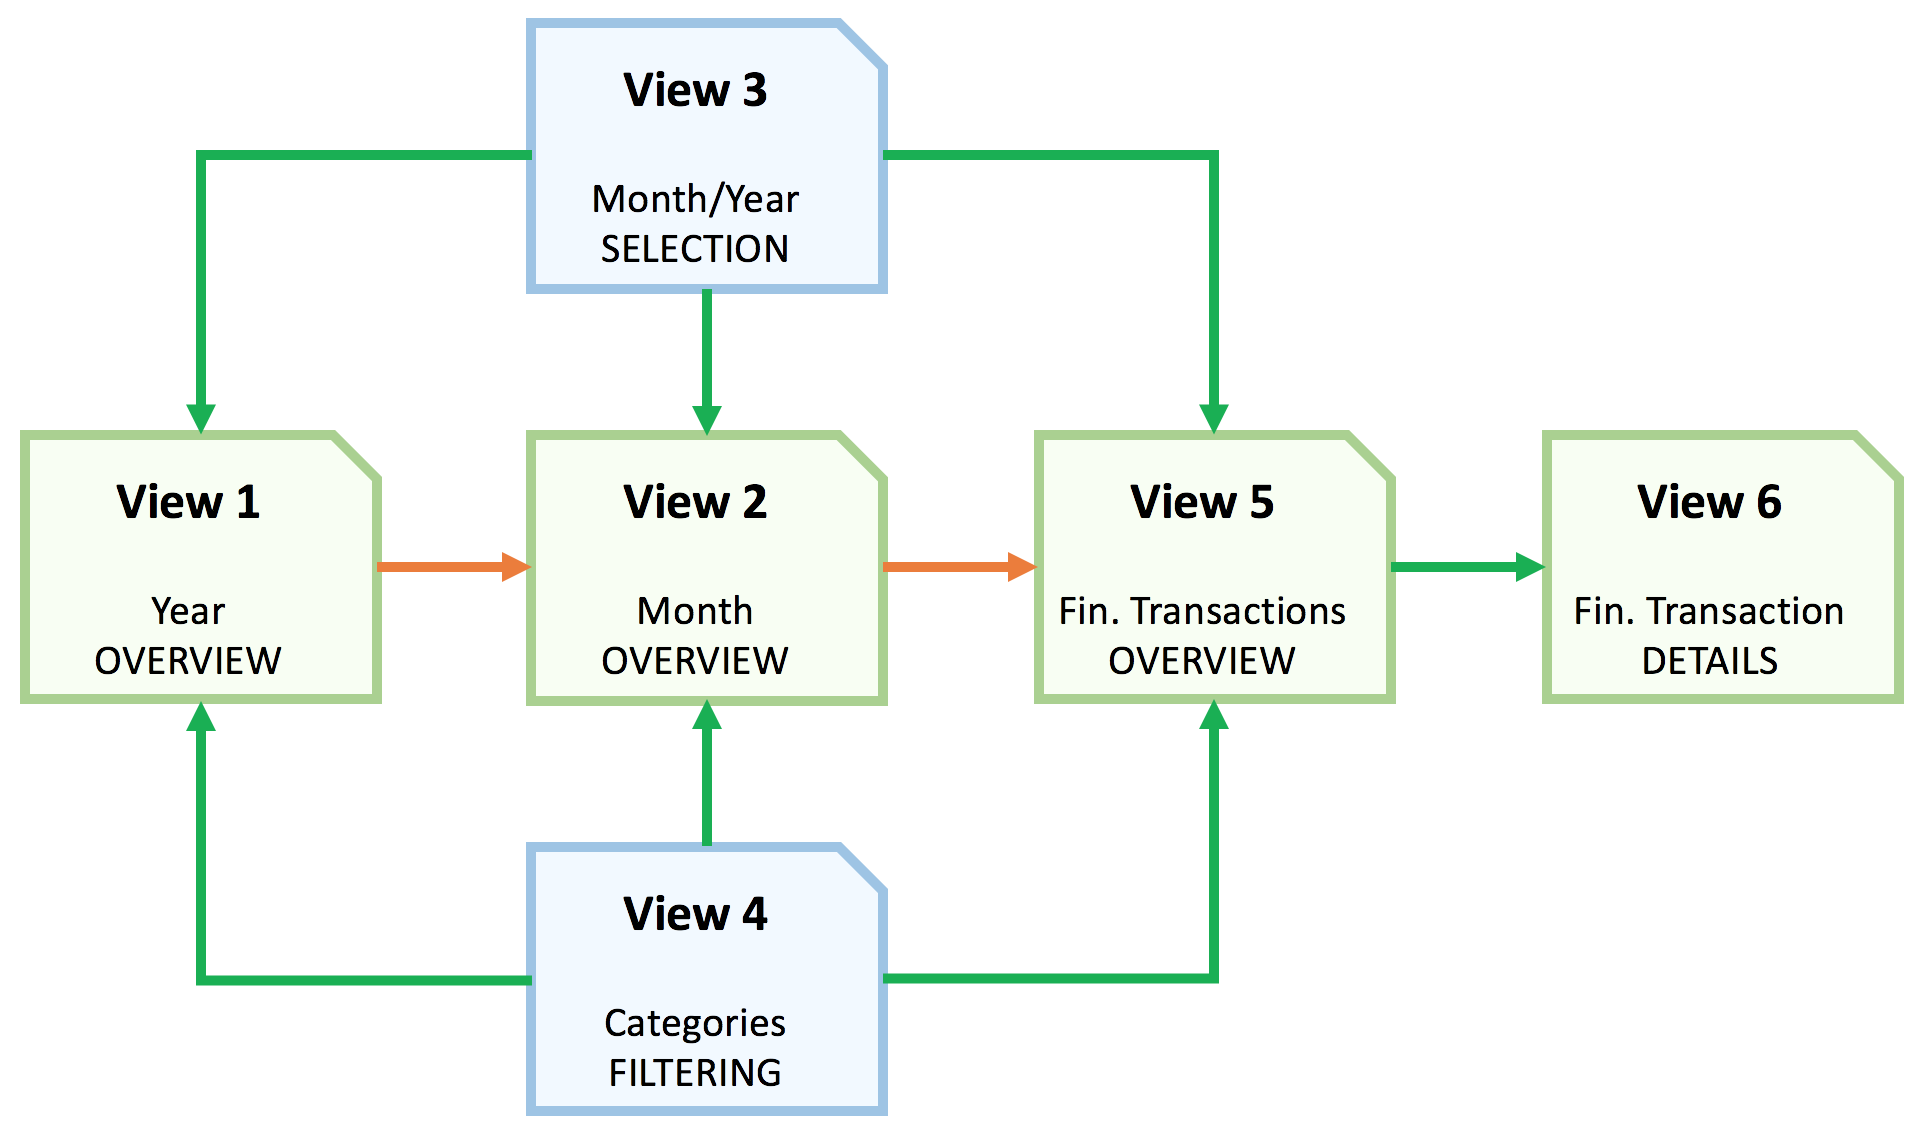
\includegraphics[width=14cm]{03_Figures/07_Suggestion/NavigationMap.png}
		\caption{Navigation Map of Design Suggestion}
		\label{fig:navigationmap}
	\end{center}
\end{figure}

For a better understanding, in Table \ref{tbl:navigationmap} each navigation flow is explained in more detail.
\begin{longtable}{ | p{2.5cm} | p{11.5cm} |}
	\hline
	\textbf{Flow} & \textbf{Description} \\
	\hline
	\endfirsthead % Line(s) to appear as head of the table on the first page
	\multicolumn{2}{c}%
	{\tablename\ \thetable\ -- \textit{Continued from previous page}} \\
	\hline
	\textbf{Flow} & \textbf{Description} \\
	\hline
	\endhead % Line(s) to appear at top of every page (except first)
	\hline
	\multicolumn{2}{r}{\textit{Continued on next page}} \\
	\endfoot % Last line(s) to appear at the bottom of every page (except last)
	\endlastfoot % Last line(s) to appear at the end of the table
	\hline
	View 1 \textrightarrow{} 2 &
	\textbf{From} Year OVERVIEW \textbf{to} Month OVERVIEW \newline
	This main navigation flow allows the selection of a specific month, directly from the display of the year overview to update the month overview. \\
	\hline
	View 2 \textrightarrow{} 5 &
	\textbf{From} Month OVERVIEW \textbf{to} Fin. Transactions OVERVIEW \newline
	The second main navigation flow enables the selection of an individual day, directly from the display of the month to apply an additional filter on view 5. \\
	\hline
	View 3 \textrightarrow{} 1 \newline
	View 3 \textrightarrow{} 2 &
	\textbf{From} Year SELECTION \textbf{to} Year OVERVIEW \newline
	\textbf{From} Year SELECTION \textbf{to} Month OVERVIEW \newline
	With the selection of a different year, the displayed data in the month/year overview will be updated accordingly. \\
	\hline
	View 4 \textrightarrow{} 1 \newline
	View 4 \textrightarrow{} 2 &
	\textbf{From} Categories FILTERING \textbf{to} Year OVERVIEW \newline
	\textbf{From} Categories FILTERING \textbf{to} Month OVERVIEW \newline
	By changing the categories filter, the displayed data in the month/year overview is updated based on the new filter. \\
	\hline
	View 4 \textrightarrow{} 5 &
	\textbf{From} Categories FILTERING \textbf{to} Fin. Transactions OVERVIEW \newline
	By changing the categories filter, the list of financial transactions is also updated to reflect the new filter selection. \\
	\hline
	View 5 \textrightarrow{} 6 &
	\textbf{From} Fin. Transactions OVERVIEW \textbf{to} Fin. Transaction DETAIL \newline
	By selecting a single transaction from the list, the corresponding detail information are shown. \\
	\hline
	\caption{Explanation of the different flows in the navigation map}
	\label{tbl:navigationmap}
\end{longtable}


%-----------------------------------
%	SUBSECTION 3
%-----------------------------------

\subsection{Conclusion}

With the implementation of real \textit{Multi View} in \gls{vr}, the focus of \textit{Zoom In} is limited to the selection of an individual transaction from a list, whereas the \textit{Zoom Out} is not required anymore at all. Furthermore, by updating all main views simultaneously when changing the selection or filter helps to cover the \textit{Relate} task, especially when also additional visualisation clues are in place. These are covered in the next sub-chapter.


%----------------------------------------------------------------------------------------
%	SECTION 4
%----------------------------------------------------------------------------------------

\section{Visualisation of Views and Data}

As already indicated in the previous chapters, \gls{vr} allows for a lot more space to visualize objects compared to regular 2D space. This opportunity has to be seized and thus the previously defined views can be displayed next to each other, similar to what has been done by \cite{CodeScience2015} and is shown in Figure \ref{fig:rotatingringstoweranddetail} in Chapter \ref{SubSectionRotatingDataRings}. The somewhat natural flow from left to right in Figure \ref{fig:navigationmap} can also be applied into the \gls{ve}. \newline
The individual views are discussed in the following sub-chapters with a conclusion at the end.


%-----------------------------------
%	SUBSECTION 1
%-----------------------------------

\subsection{View 1: Year Overview}

This view should give the user an impression about the changes in the financial expenses over the course of a whole year. Since the data set is more logically structured than the example data that has been used by \cite{Jamieson2007} for their implementation of a 'Data Forest', it would only provide limited usability. Their approach could make sense when the individual transactions were shown as trees in a forest. While this would provide a new insight in the distribution of all expenses, it does not give an easy to understand view on the (financial) situation of the year as a total, especially since the transactions are also categorized. \newline
Alternatively, a more traditional approach can be chosen where the data is visualized in ways that are well-known to most people, such as a line or bar chart. \cite{Drouhard2015} emphasized that a full transition to a 3D environment can be difficult wherefore the focus should be rather put on the question how 2D interactions can be brought into 3D space in the most effective way. Since this overview will only contain little information (i.e. an amount sum per month), the potential problems with scaling of large data as indicated by \cite{Jamieson2007} can be neglected in this scenario. Such a traditional visualisation solution also is beneficial for first-time users as they immediately see something familiar that they can relate to. \cite{Wann1996} stated on this topic that the goal in building \glspl{ve} is to minimize the learning required to operate within them, but at the same time maximize the information yield. Building up on this, \cite{Burlutskiy2014a} said that aesthetically attractive visualisation don't necessarily allow for a good reasoning by the user, especially when the visualisation does not explicitly visualize the categories in which the user is interested in. This further emphasizes the need to rely on well-known visualisation techniques to make it as simple as possible for a user to intuitively know what to do. \newline
To allow a more diverse manipulation of the individual month (objects), the bar chart provides more possibilities compared to a line chart that has only single points. In the vertical axis, the summarized totals are displayed, whereas in the horizontal axis the individual months are listed. As an additional information to the user, a 'plan-value' line can also be shown to more easily indicate in which months the spendings are above/below the planned expenses. By changing the colours of the individual bars, this information can be brought to the users attention much more effectively. Figure \ref{fig:view1chart} shows exemplary how such a chart could look like in 2D, where the red values indicate the amounts above the planned value.
\begin{figure}[h]
	\begin{center}
		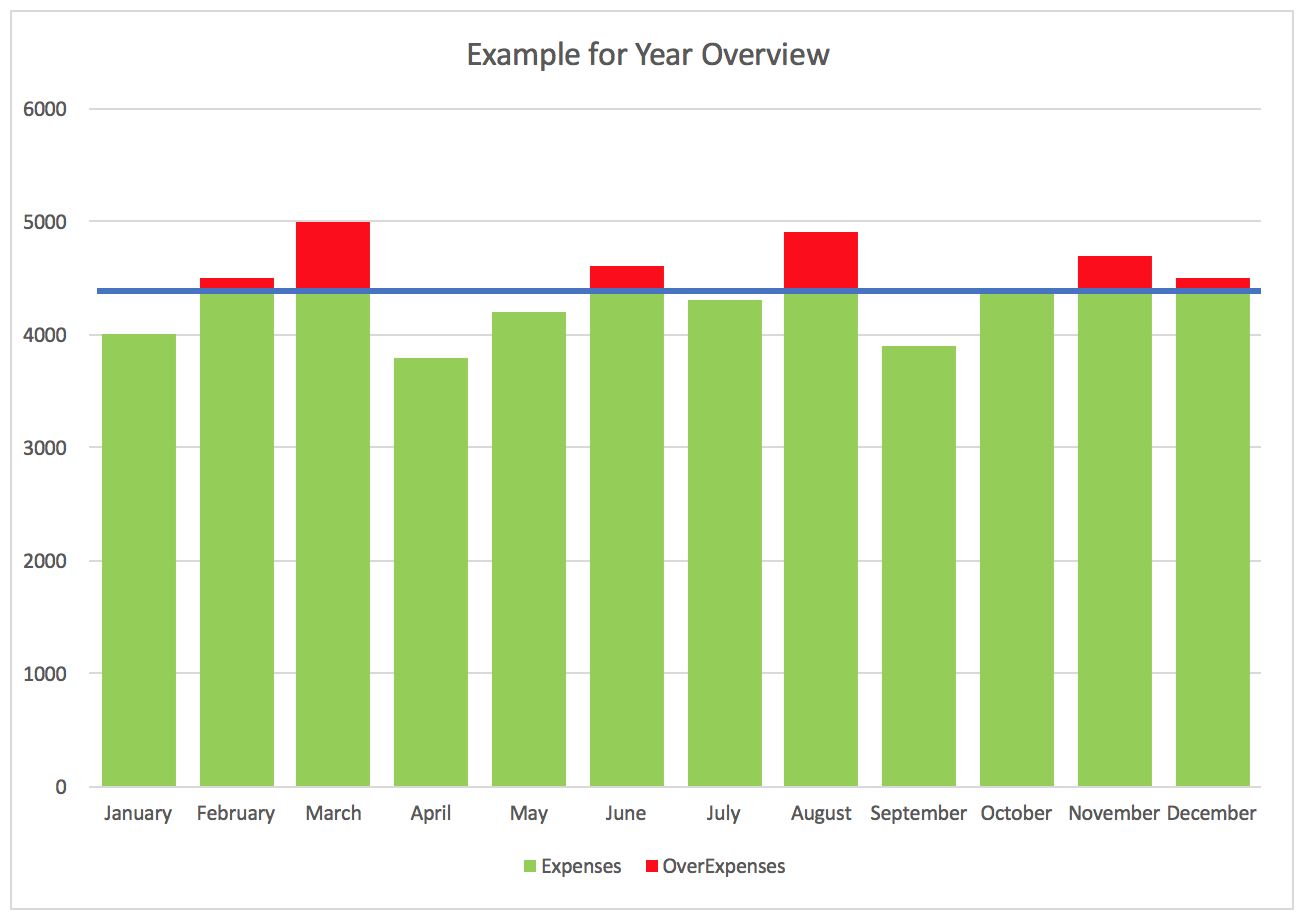
\includegraphics[width=14cm]{03_Figures/07_Suggestion/View1_YearOverview.png}
		\caption{Exemplary visualisation of View 1: Year Overview}
		\label{fig:view1chart}
	\end{center}
\end{figure}
If also a specific month has been selected, it can be visually highlighted in this view to keep all of them synchronized. This is in accordance with the findings of \cite{Hentschel2009}, which showed that multiple linked views can be a very good solution for the interactive analysis of time-dependent data, like it is the case here.


%-----------------------------------
%	SUBSECTION 2
%-----------------------------------

\subsection{View 2: Month Overview}

The second view is similar to the first one as it also shows a temporal overview of the expenses. This time however for a single month, where the horizontal axis shows the individual days of that month. Since now on a much smaller scale, depending on the category there potentially are only very few transactions or even only a single one like for the monthly rent. This makes the visualisation of an average line like in View 1 (Year Overview) not very useful and a different approach has to be found. \newline
Alternatively, a cumulative chart where the amounts of the previous days are always added to the future days as well, could make much more sense. This would then also again allow to show an average line (of the other months) to indicate from which day onwards the average spending has been exceeded. The same colouring approach like in the previous view can be applied to give an easy to see visual cue about the situation. Figure \ref{fig:view2chart} again shows exemplary how such a chart could look like in 2D.
\begin{figure}[h]
	\begin{center}
		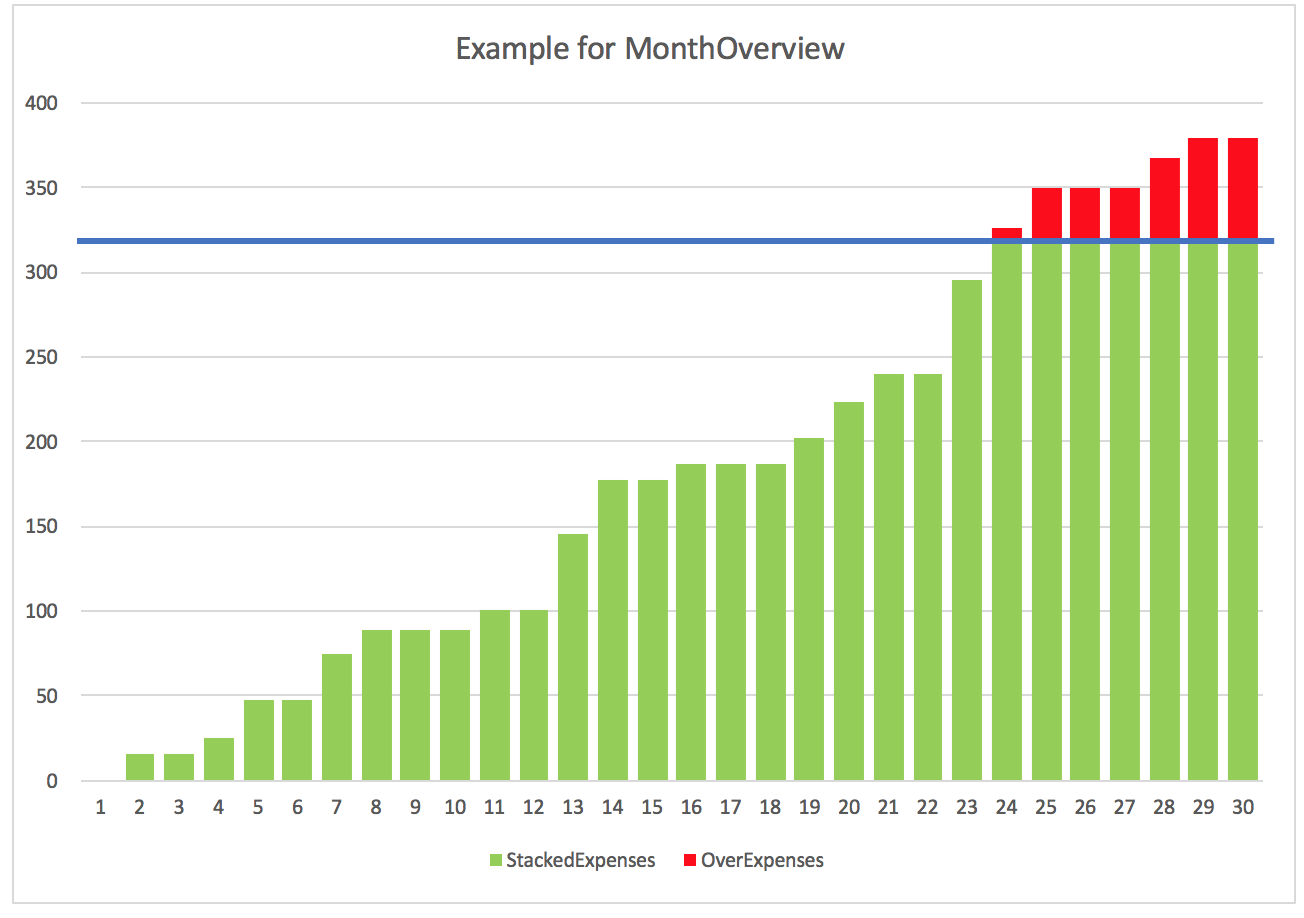
\includegraphics[width=14cm]{03_Figures/07_Suggestion/View2_MonthOverview.png}
		\caption{Exemplary visualisation of View 2: Month Overview}
		\label{fig:view2chart}
	\end{center}
\end{figure}
Like in the previous view, when an individual day is selected for the filtered list of transactions (View 5), the selection is also done visually on this chart.


%-----------------------------------
%	SUBSECTION 3
%-----------------------------------

\subsection{View 3: Year Selection}

The first support view does not really display any data-related information, but can primarily be seen as a 'date picker' view that supports the selection of individual years. It should be held as simple as possible to avoid any unnecessary interaction steps but still allows the user to intuitively select the desired high-level time-frame. Figure \ref{fig:view3chart} shows exemplary how such a selection view could look like. In this example, the currently selected year is 2016, highlighted in green colour.
\begin{figure}[h]
	\begin{center}
		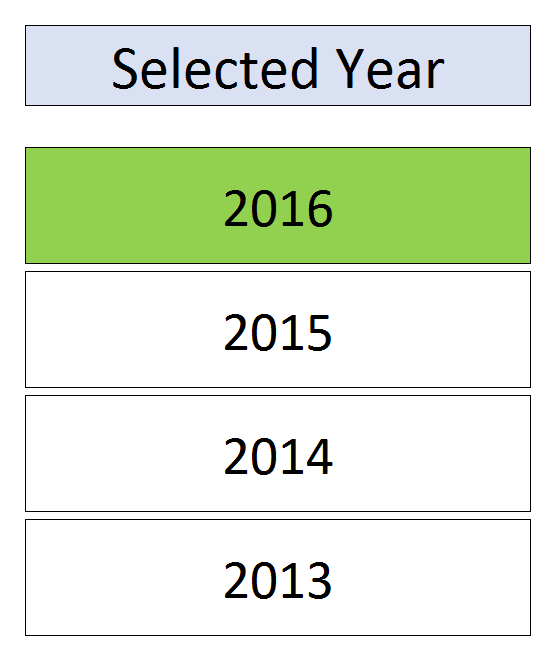
\includegraphics[width=6cm]{03_Figures/07_Suggestion/View3_YearSelection.png}
		\caption{Exemplary visualisation of View 3: Year Selection}
		\label{fig:view3chart}
	\end{center}
\end{figure}

%-----------------------------------
%	SUBSECTION 4
%-----------------------------------

\subsection{View 4: Categories Filtering}

\label{SubSectionCategoriesFiltering}

Since the filtering for the categories is applied on the selected data (compared to changing the month/year selection which 'resets' the currently selected data), it should be always in front of the user for easy access. While this could be done in some kind of pop-up menu or similar, \cite{Bowman2002} reminds us that these techniques are far less natural and could require some training for the user, especially when it is not clear that such a pop-up menu exists and how it can be displayed. Instead, and also in accordance with \gls{mdg} 3, the filtering is intended for \gls{vr} and thus should also be done in 3D. The main categories that are listed in Table \ref{tbl:financialcategories} already have some icons assigned to them in the UBS e-banking, and are shown more detailed in Figure \ref{fig:categoriesicons}. The sub-categories will not be considered for this view as their number is too high for an easy-to-understand visualisation, as well as the amount of transactions will further decrease the more low-level filtering is possible.
\begin{figure}[h]
	\begin{center}
		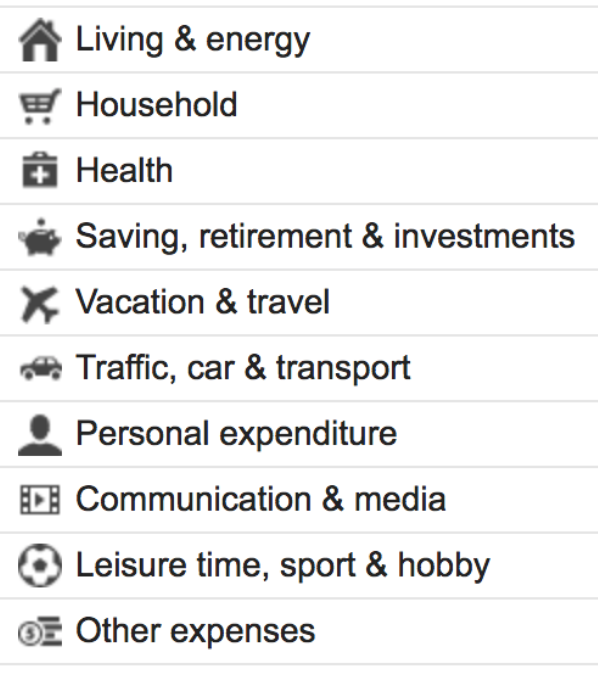
\includegraphics[width=6cm]{03_Figures/07_Suggestion/UBSAG2016_CategoriesIcons.png}
		\caption[Mapping of icons to categories in UBS e-banking demo]{Mapping of icons to categories in UBS e-banking demo \citep{UBSAG2016}}
		\label{fig:categoriesicons}
	\end{center}
\end{figure} \newline
In relation to the research done by \cite{Jamieson2007} that showed the effectiveness of familiar 3D objects for \gls{vr}, these icons can also be represented as 3D objects on a table or similar in front of the user. Depending on whether a certain category/object is enabled for the filtering, its colour can change from e.g. green (enabled) to white (disabled), similar to how this is done by \cite{LeapMotion2016} in their demo 'Geometric' as shown in Figure \ref{fig:leapmotiongeometric} where the right-most button is active (yellow) and the other two are inactive (white).
\begin{figure}[h]
	\begin{center}
		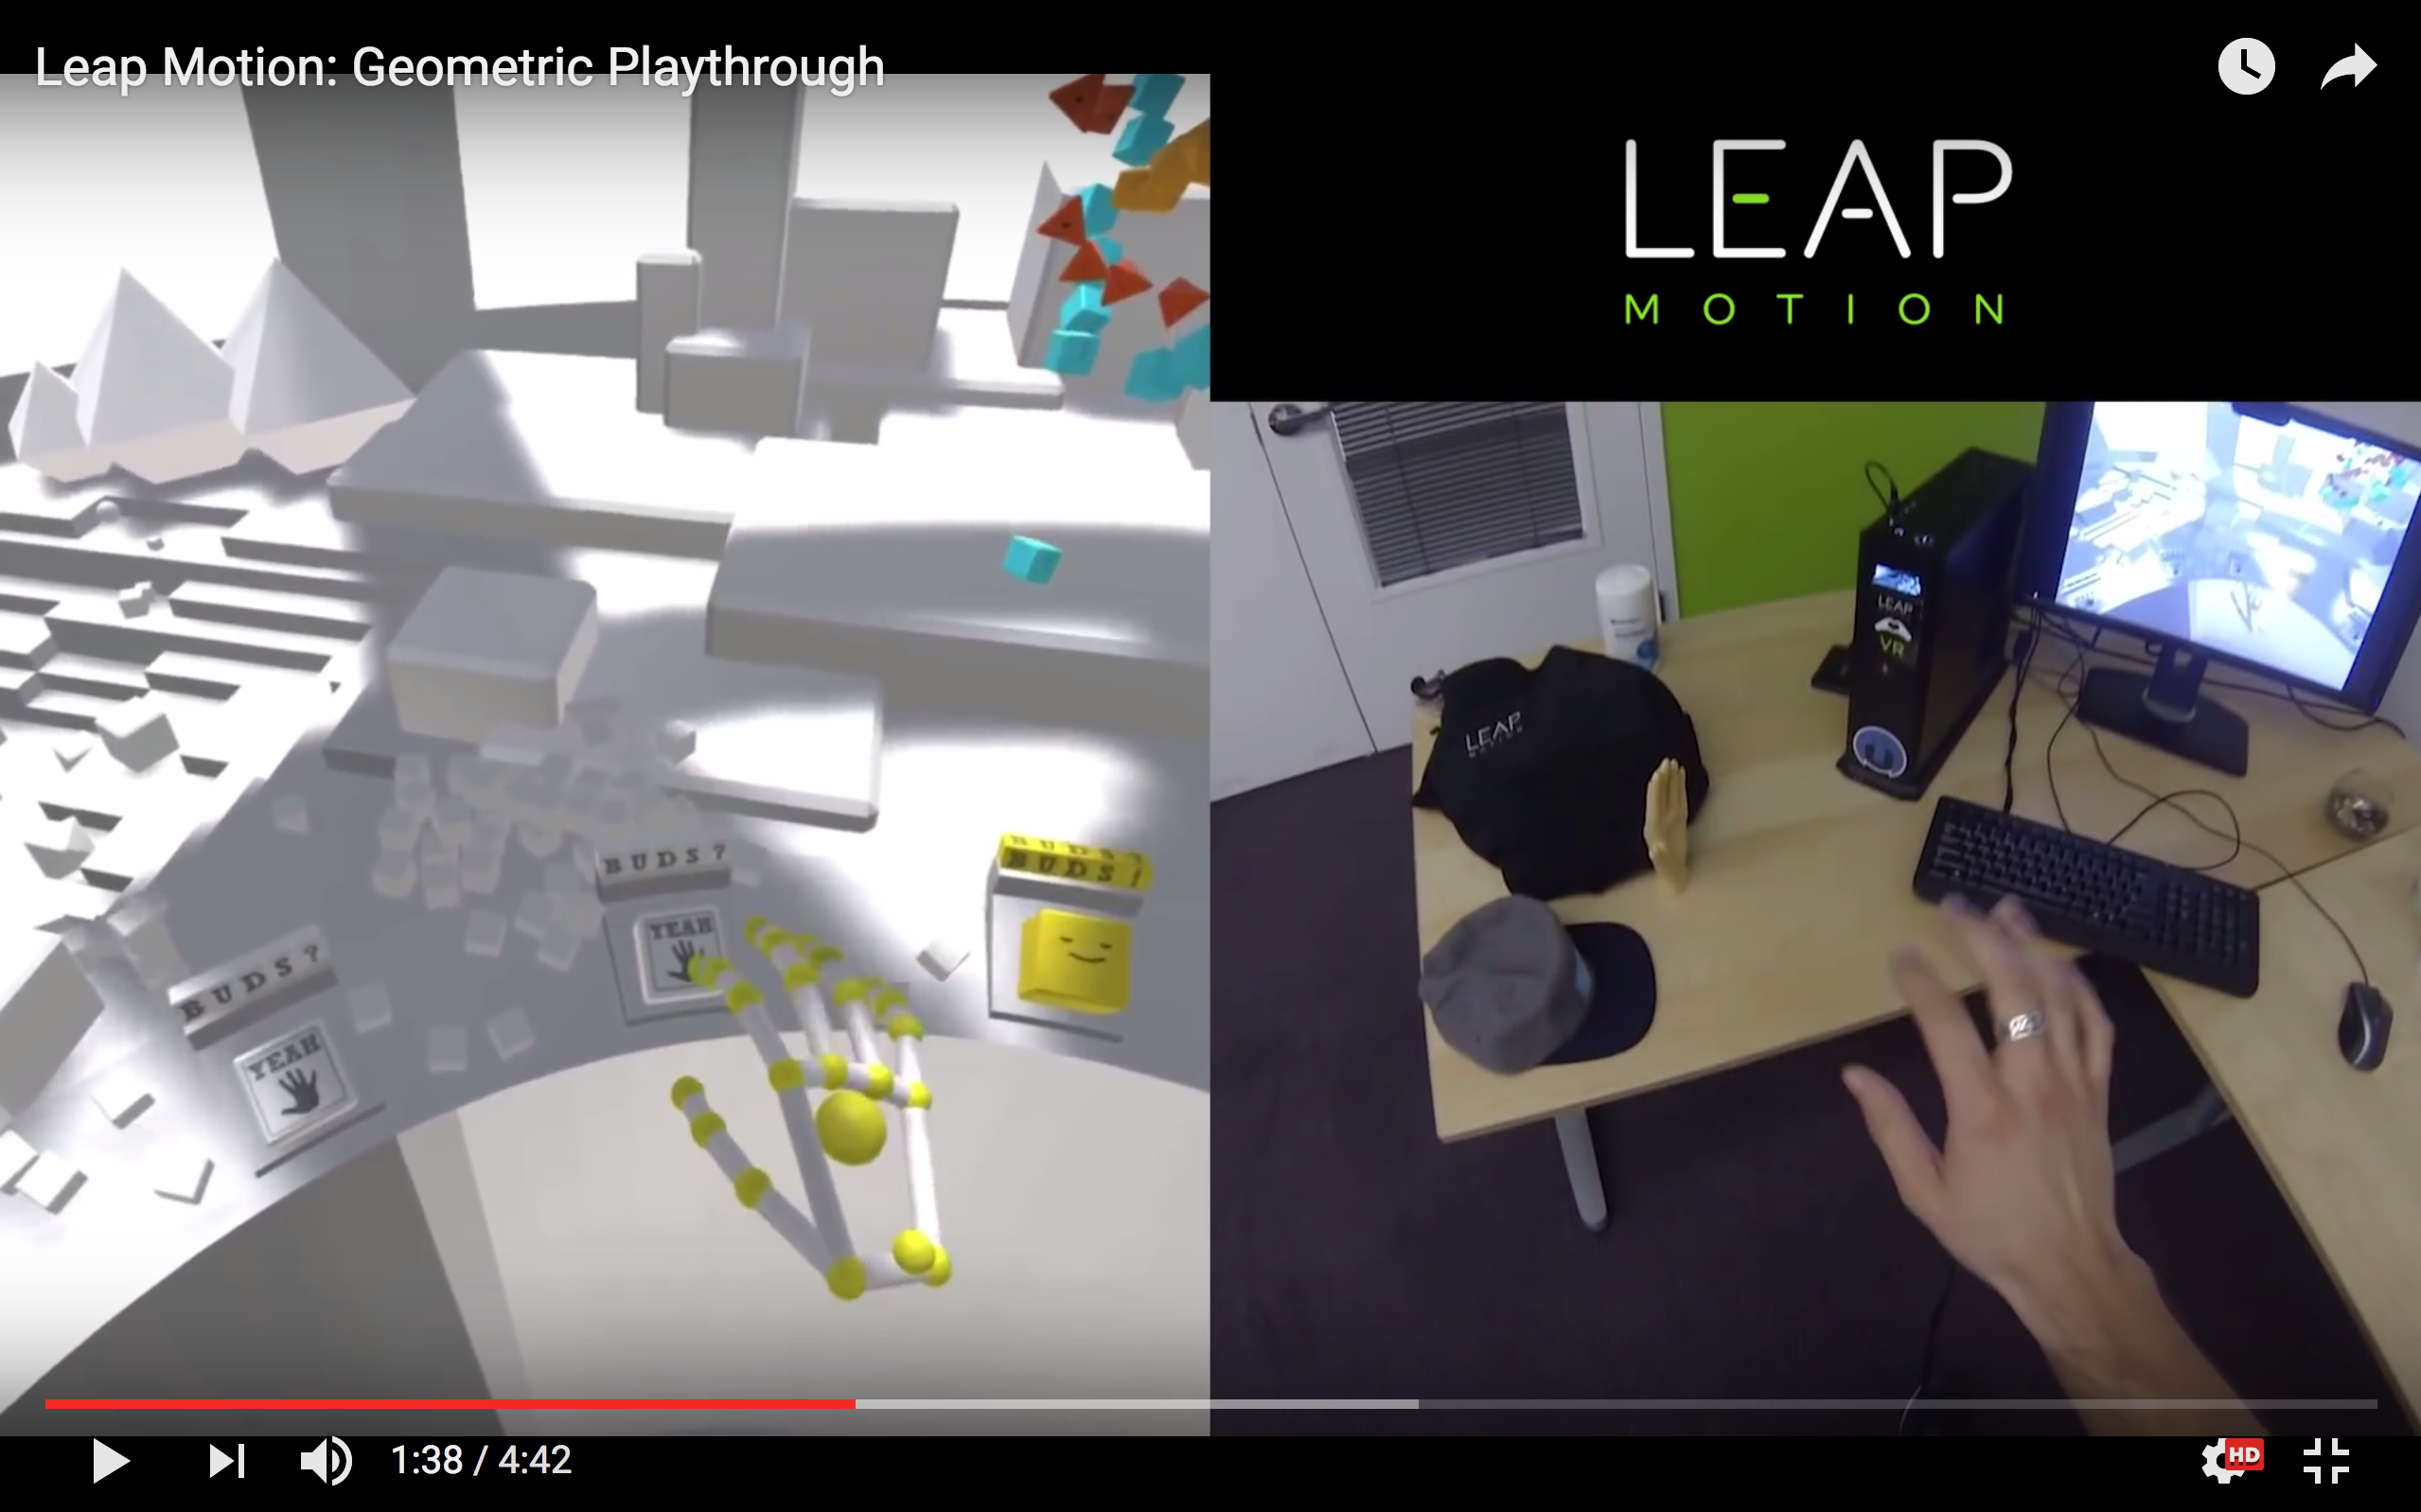
\includegraphics[width=14cm]{03_Figures/07_Suggestion/LeapMotion2016_Geometric.png}
		\caption[Different button states in Leap Motion demo 'Geometric']{Different button states in Leap Motion demo 'Geometric' \citep{LeapMotion2016}}
		\label{fig:leapmotiongeometric}
	\end{center}
\end{figure}


%-----------------------------------
%	SUBSECTION 5
%-----------------------------------

\subsection{View 5: Financial Transactions Overview}

Although this fifth view is defined as an 'overview', it already provides rather detailed information about the individual transactions. At this point, the user is interested in the raw data due to which the use of 3D objects will be very limited. This view has to provide enough information to understand what the individual transactions were about, but still only show as little as necessary to not overcomplicate the data table. Absolutely necessary are the date of the transaction, the amount and currency, the recipient, and presumably also the category to which it belongs. This can also help the user to directly see which additional filters he might have to apply to narrow down his exploratory research in the way he wants to. For a more detailed view on a single transaction, where all other information can be displayed, View 6 will be the place to navigate to.


%-----------------------------------
%	SUBSECTION 6
%-----------------------------------

\subsection{View 6: Financial Transaction Detail}

On the lowest level, the details about one single financial transaction are displayed. Additional information such as the booking text, the account number/name from which the payment was made, or also the subcategory can be displayed. Similar to the detailed data in the 'Rotating Data Rings' implementation of \cite{CodeScience2015} shown in Figure \ref{fig:rotatingringstoweranddetail}, the pure raw data will be presented in this view in the structure of a simple grid. \newline
By referring back to the main task 'Relate' from the \gls{vism} 2.0, with the highlighted entries in the other views, a clear link to the relationship of this single entry can be drawn to the month overview and the year overview.


%----------------------------------------------------------------------------------------
%	SECTION 5
%----------------------------------------------------------------------------------------

\section{Mapping of Interaction Patterns}

After the definition of the individual views, the interaction patterns can be mapped to them. As discussed in Chapter \ref{SubSectionInteractionPatterns}, there are three main types of interaction patterns: Travel, Selection, and Manipulation. As defined in \gls{mdg} 1, high interactivity is one of the main design goals for this artefact, which will be a key component in the following sub-chapters when the three interaction pattern types are discussed in more detail. This design goal is also heavily linked to the concept of 'multiple linked views' of \cite{Hentschel2009} which has proven to be very useful when dealing with temporal data.

%-----------------------------------
%	SUBSECTION 1
%-----------------------------------

\subsection{Travel}

The simplest interaction pattern is \textit{Travel}. In accordance with \gls{mdg} 2 which states that the user us part of the \gls{ve} and thus us able to 'travel' around the visualisation, theoretically any kind of locomotion would be applicable. Due to the fact, that the different views are presented around or in front of the user and they are only of very limited number, there is no direct need for any kind of teleportation functionality. While a 'seated' \gls{vr} experience is more limited, it does not prevent the user from viewing all relevant views. A 'room-scale' experience on the other hand provides some more freedom especially in terms of 'Zoom In' and 'Zoom Out' as the user can walk closer or further away from it.


%-----------------------------------
%	SUBSECTION 2
%-----------------------------------

\subsection{Selection}

The \textit{Selection} pattern is undeniably the most important one since the core activity is data exploration. For a better understanding, Figure \ref{fig:interactionmap} gives an overview of all views and their interaction paths that have been numbered. The following list will give some more detailed information on what exactly happens on the different interaction paths.
\begin{figure}[h]
	\begin{center}
		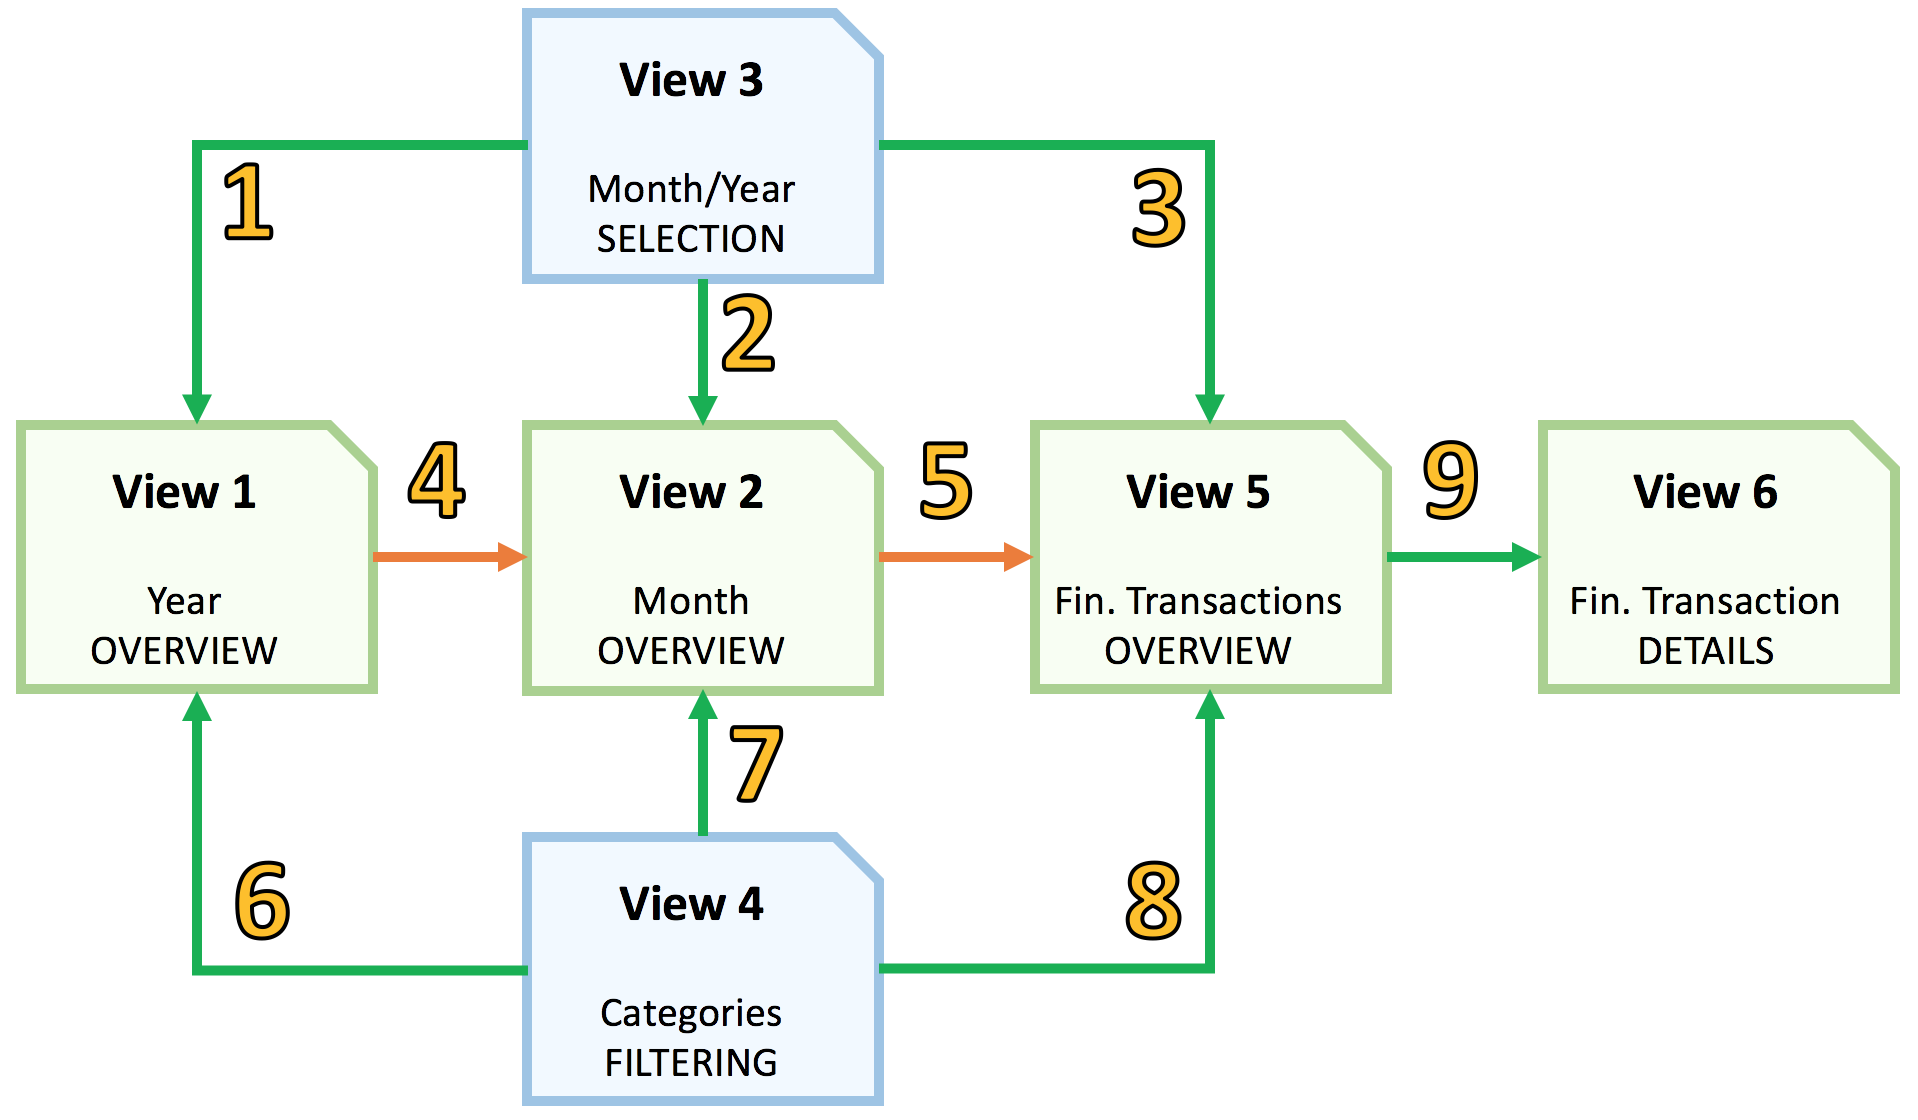
\includegraphics[width=14cm]{03_Figures/07_Suggestion/InteractionMap.png}
		\caption[Interaction Map of Design Suggestion]{Interaction Map of Design Suggestion (based on Figure \ref{fig:navigationmap})}
		\label{fig:interactionmap}
	\end{center}
\end{figure}

\textbf{Path 1: View 3 \textrightarrow View 1} \newline
When selecting a different year, this will trigger an update on the Year Overview where now all data for the selected year will be displayed. Any filter applied in view 4 will also influence the final data that is displayed.

\textbf{Path 2: View 3 \textrightarrow View 2} \newline
When selecting a different year, this will trigger a clear of the Month Overview, as first a specific month needs to be selected again from the Year Overview.

\textbf{Path 3: View 1 \textrightarrow View 2} \newline
From within the Year Overview it is also possible to trigger a month change by selecting one of the 'bars' in the chart. In addition to that, it will also trigger the next interaction path (no. 4) and update the list of financial transactions that are displayed.

\textbf{Path 4: View 2 \textrightarrow View 5} \newline
Similar to Path 3, it is also possible to select the 'bar' of a single day to trigger an update on the list of financial transactions. This path can also be indirectly triggered when a month is selected in the Year Overview. This will also trigger Path 8 as any previously selected single transaction will be cleared from the view.

\textbf{Path 5: View 4 \textrightarrow View 1} \newline
Compared to Path 1, this is an additional (data) filter that is applied on the selected data set from View 3. Individual categories can be enabled and disabled. \textit{Note: A change in View 4 will always trigger all three interaction paths: 5, 6, and 7.}

\textbf{Path 6: View 4 \textrightarrow View 2} \newline
Very similar to Path 5, this is an additional (data) filter that is applied on the selected data set from View 3. \textit{Note: A change in View 4 will always trigger all three interaction paths: 5, 6, and 7.}

\textbf{Path 7: View 4 \textrightarrow View 3} \newline
Again, the list of transactions will be updated by applying this additional (data) filter. This will also trigger Path 8 as any previously selected single transaction will be cleared from the view. \textit{Note: A change in View 4 will always trigger all three interaction paths: 5, 6, and 7.}

\textbf{Path 8: View 5 \textrightarrow View 6} \newline
The final path is triggered when a single transaction is selected from the list in view 5. This path is also triggered whenever the list is updated and will cause the view to be cleared.



%-----------------------------------
%	SUBSECTION 3
%-----------------------------------

\subsection{Manipulation}

Direct \textit{Manipulation} of the underlying data set itself is not possible in this design, as it focuses on the exploratory aspect. However, there is a direct manipulation possibility for 3D objects in one of the views.
\textbf{View 4: Categories Filtering} \newline
As defined before, the different categories are visualized as three-dimensional objects that refer to the category icons from Figure \ref{fig:categoriesicons}. Interacting with these objects allows a manipulation of their state (on/off) as well as the corresponding state colour (on = green, off = white).

All other views solely make use of \textit{Selection} and do not have any applicable \textit{Manipulation} patterns.


%----------------------------------------------------------------------------------------
%	SECTION 6
%----------------------------------------------------------------------------------------

\section{Conclusion}

In this chapter, the Design Suggestion has been defined with design goals, the navigation map, the visualisation of views and data, and the mapping of interaction patterns. Furthermore, the whole design is done hardware independent in order to comply with \gls{sdg} 1. To answer \gls{srq} 4 that asks for the added value that can be created by bringing this functionality into virtual reality, several (theoretical) benefits have been found, although they can only be confirmed upon developing and evaluation the prototype application. One major advantage can be the multiple linked views that provide easier viewing access to all relevant data as well as the advanced filtering by categories which can be done intuitively with customized 3D objects. Furthermore, the supporting views are kept to a minimum and should never prevent a clear view on the relevant data. \newline
In order to evaluate this design, the next chapter describes the \textit{Development} of the prototype which is based on this \textit{Suggestion}.
